\documentclass[aspectratio=169]{beamer}
\setbeamertemplate{navigation symbols}{}
\usepackage{color,amsmath,comment, subfigure}
\usepackage{booktabs}
\usepackage{url}

%\setbeameroption{show notes}

%%%%%%%%%%%%%%%%%%%%%%%%%%
\title[]{Lecture 3: More on the small world problem\\and some history}
\author[]{Sociology 204: Social Networks, Spring 2021}
\institute[]{Matthew J. Salganik}
\date[]{
3/3: Triadic closure on Twitter

\vfill

\begin{flushleft}
\vspace{0.7in}

\includegraphics[width=0.05\textwidth]{figures/cc.png}
\end{flushleft}
}

\begin{document}
%%%%%%%%%%%%%%%%%%%%%%%%%%%
\frame{\titlepage}
%%%%%%%%%%%%%%%%%%%%%%%%%%%
\begin{frame}

\begin{figure}
\centering
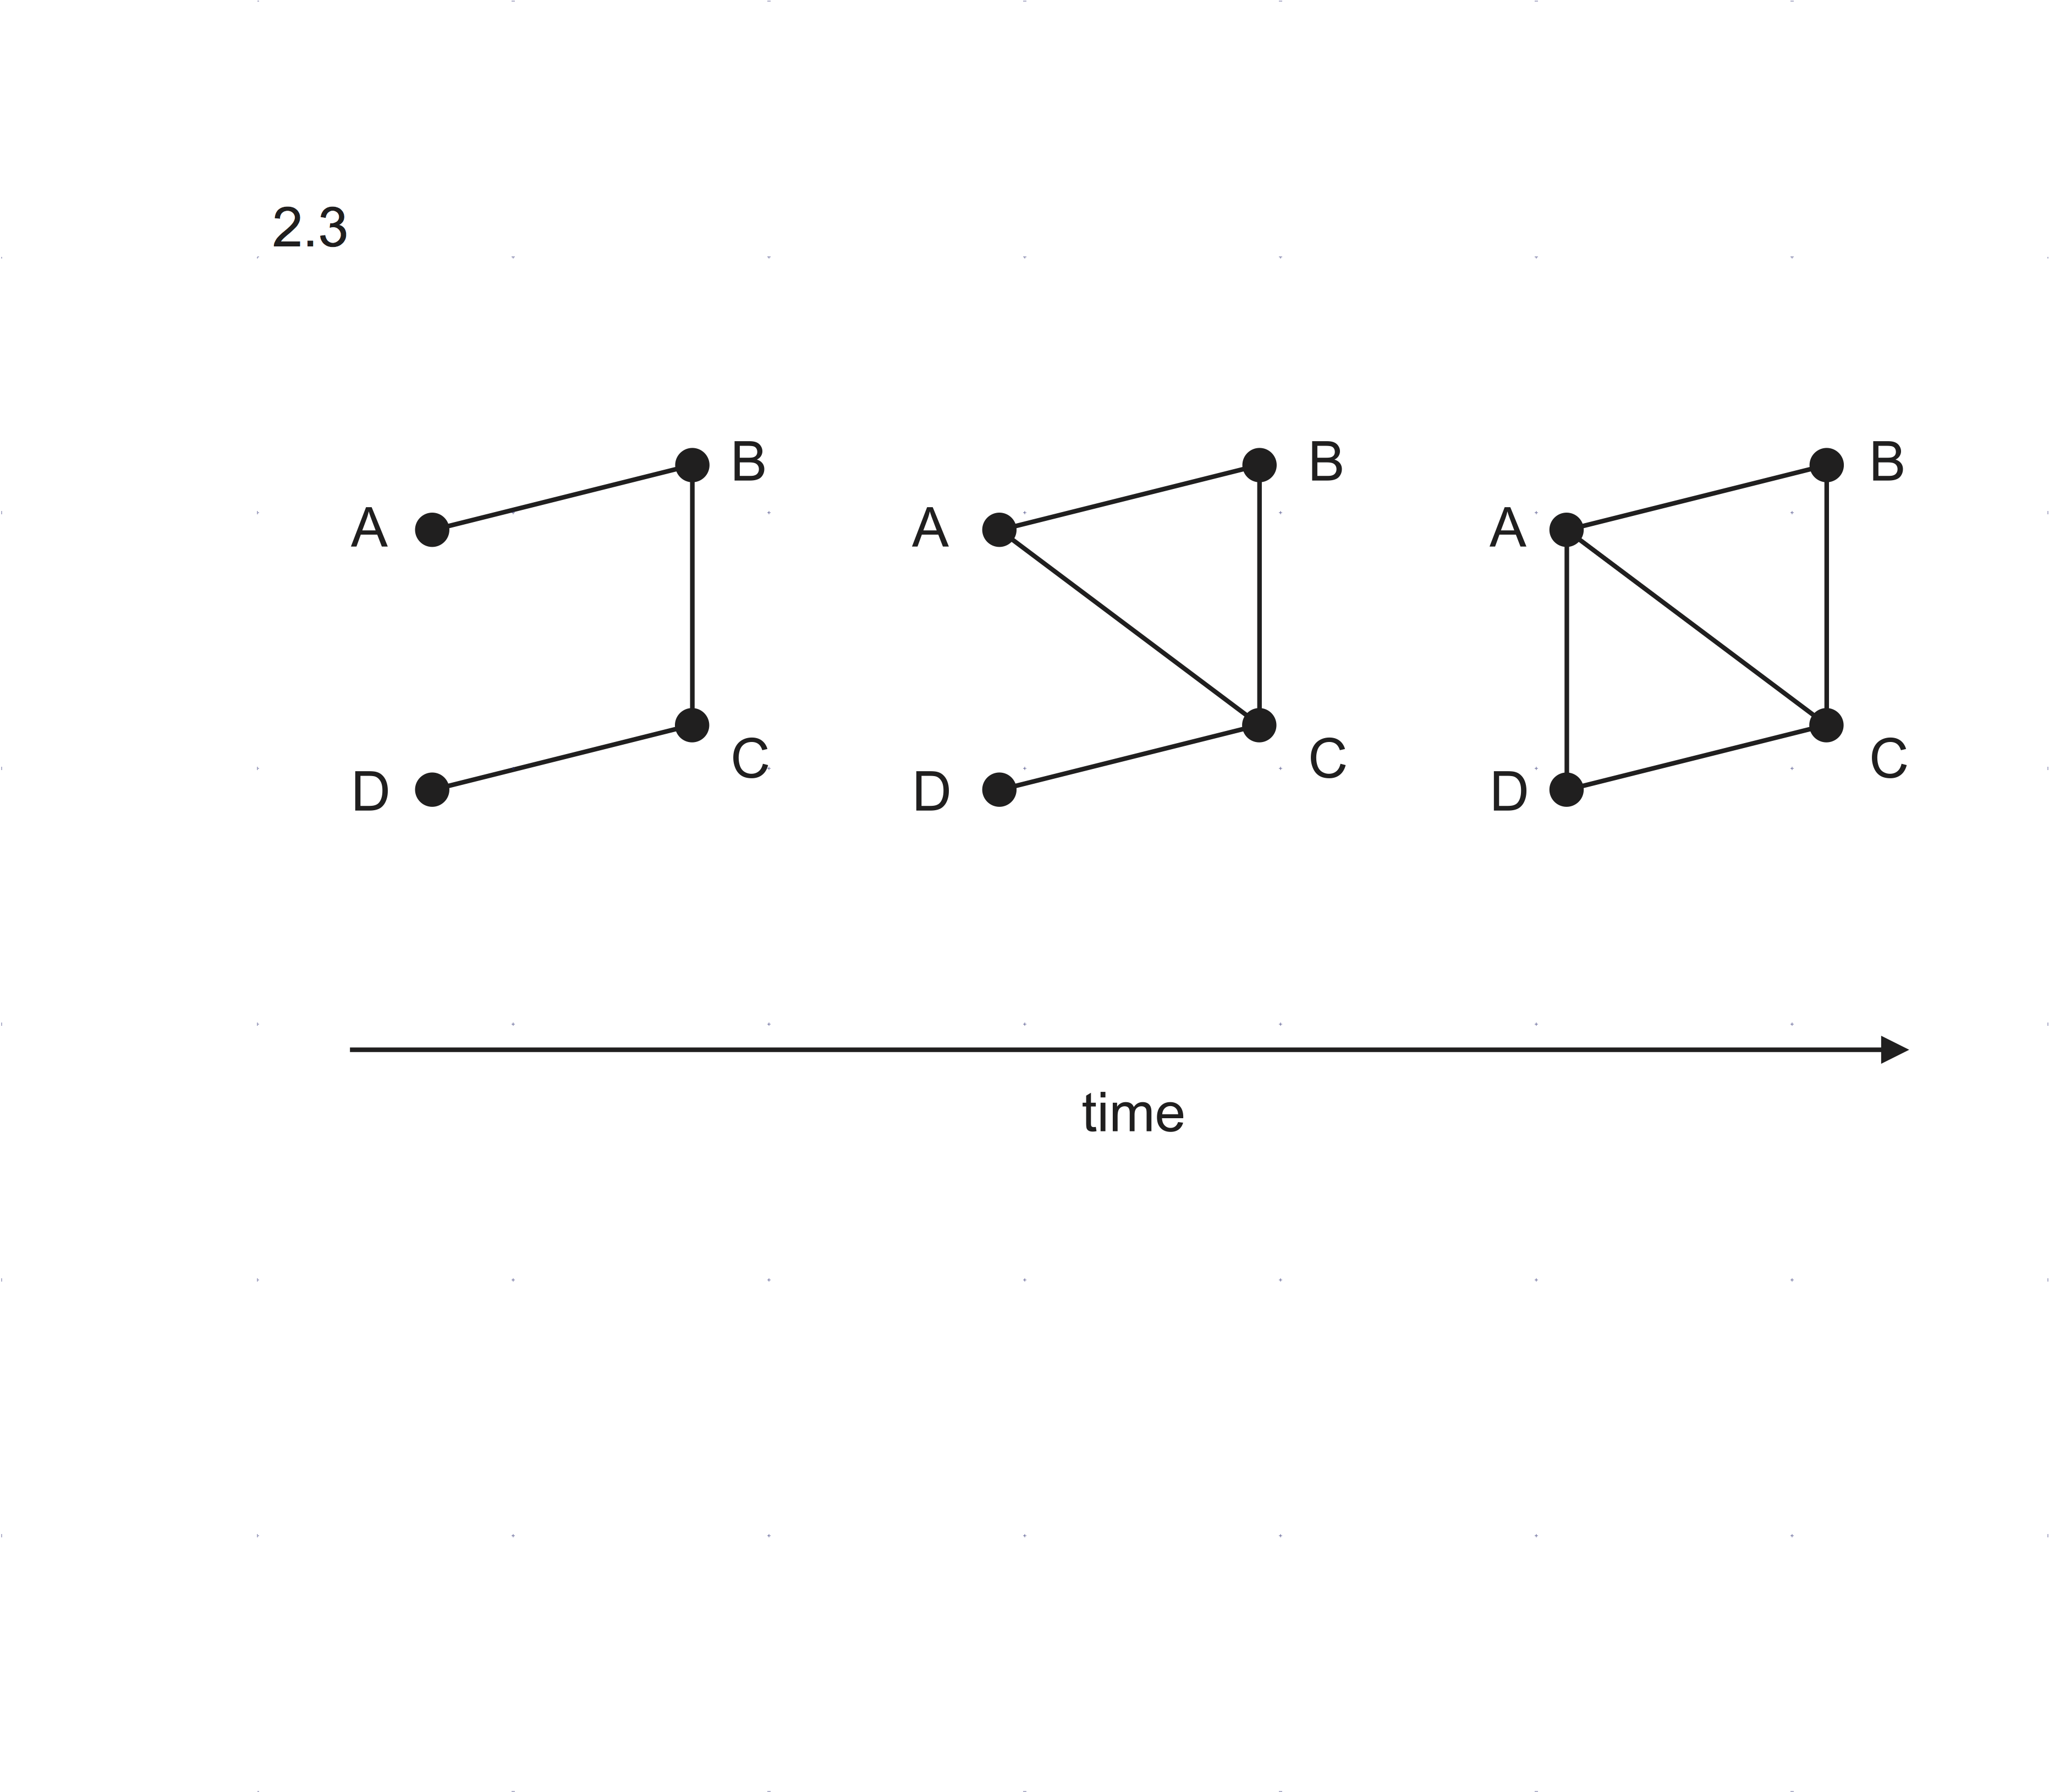
\includegraphics[width=\textwidth]{figures/2_3}
\end{figure}

\note{
Graphs grow over time through traidic closure
}

\end{frame}
%%%%%%%%%%%%%%%%%%%%%%%%%%%%
\begin{frame}

\begin{figure}
\centering
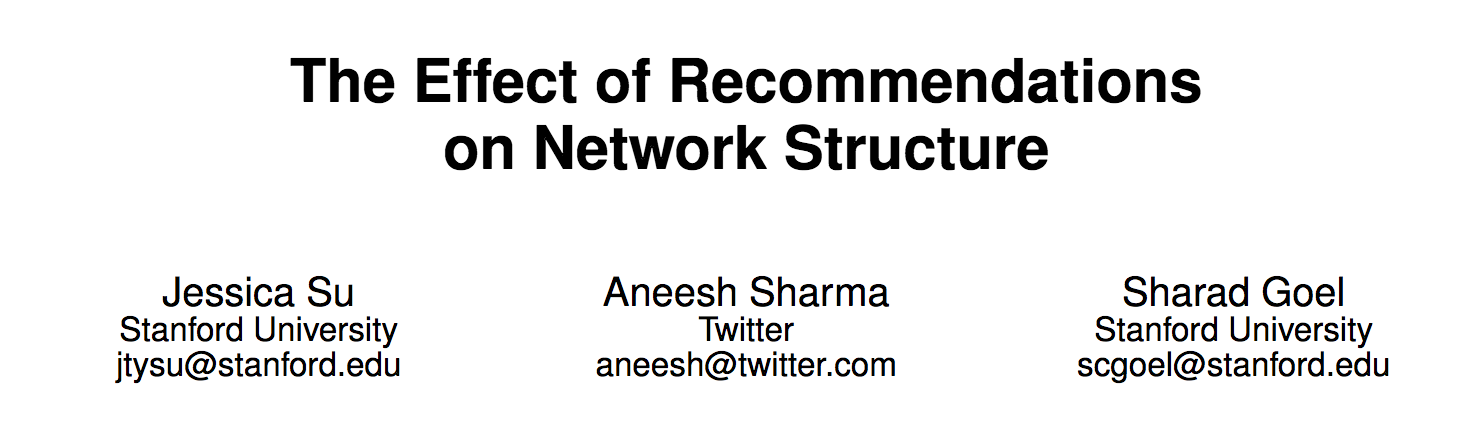
\includegraphics[width = \textwidth]{figures/su_effect_2016_title}
\end{figure}

\vfill

\url{http://dx.doi.org/10.1145/2872427.2883040}

\end{frame}
%%%%%%%%%%%%%%%%%%%%%%%%%%%%
\begin{frame}

\begin{figure}
\centering
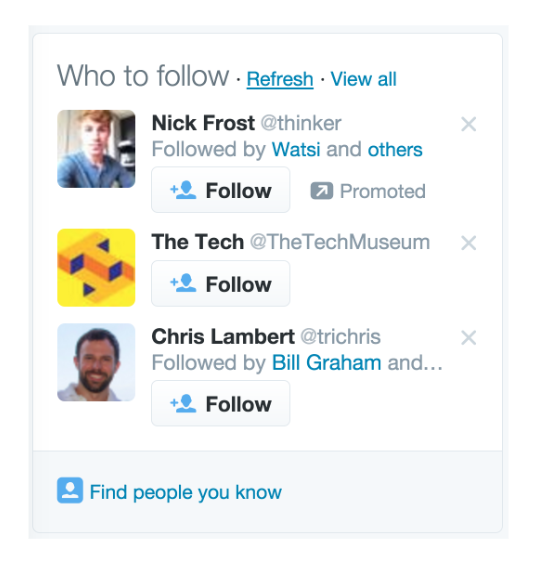
\includegraphics[height = \textheight]{figures/su_effect_2016_fig1}
\end{figure}

\end{frame}
%%%%%%%%%%%%%%%%%%%%%%%%%%%%
\begin{frame}

\begin{figure}
\centering
\includegraphics<1>[width = 0.3\textwidth]{figures/friend-of-friend-twitter_1}
\includegraphics<2>[width = 0.6\textwidth]{figures/friend-of-friend-twitter_2}
\includegraphics<3>[width = 0.6\textwidth]{figures/friend-of-friend-twitter_3}
\end{figure}


\note{
The people that the people you follow follow
Random walk to a person you follow then random walk to that person 
Good properties:
Easy computationally
More likely to recommend people more of your followers follow
}

\end{frame}
%%%%%%%%%%%%%%%%%%%%%%%%%%%%
\begin{frame}

\begin{figure}
\centering
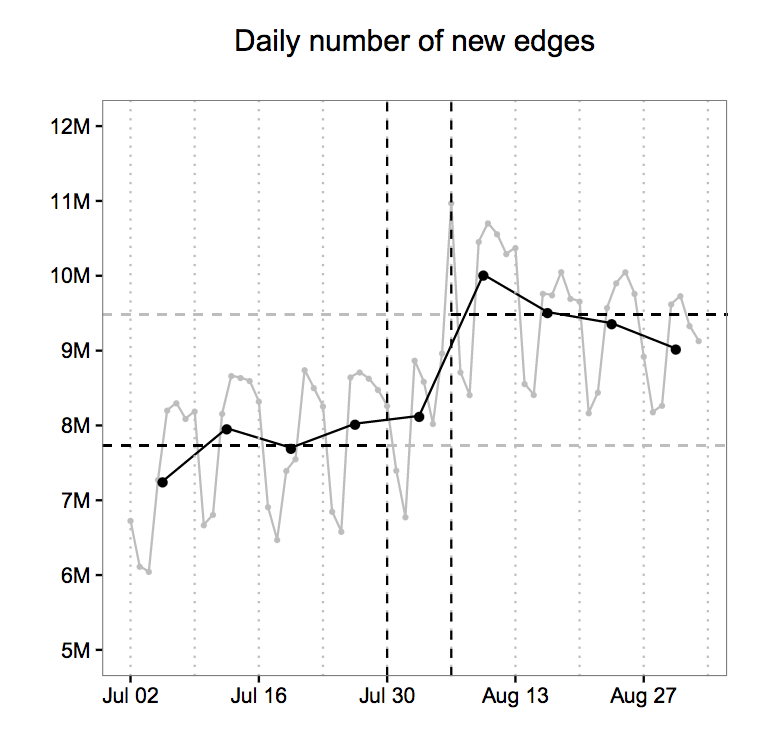
\includegraphics[height = \textheight]{figures/su_effect_2016_fig2}
\end{figure}

\end{frame}
%%%%%%%%%%%%%%%%%%%%%%%%%%%%
\begin{frame}

\begin{figure}
\centering
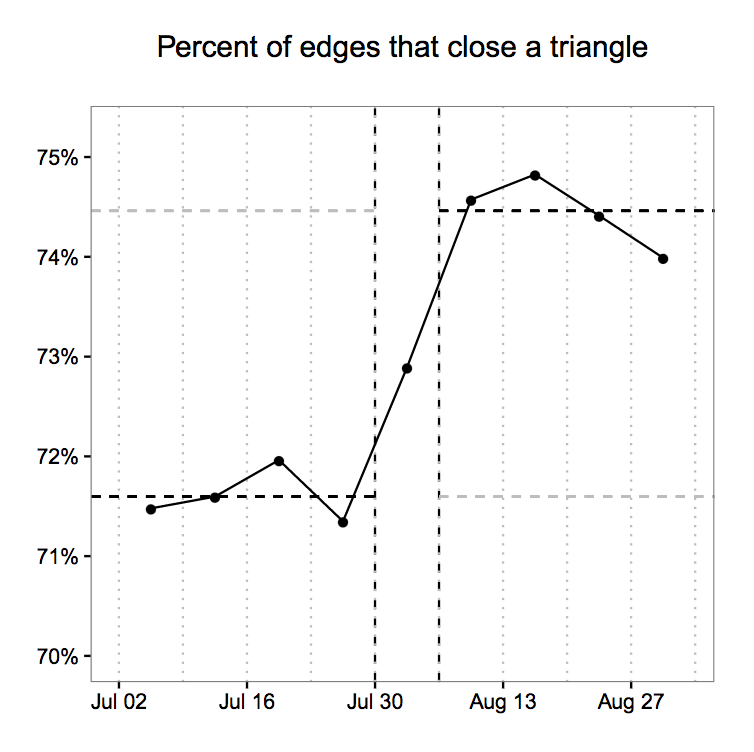
\includegraphics[height = \textheight]{figures/su_effect_2016_fig10a}
\end{figure}

\end{frame}
%%%%%%%%%%%%%%%%%%%%%%%%%%%%
\begin{frame}

Online behavior = human behavior + algorithmic bias

\note{
People who work at Facebook and Twitter took classes like this one
They have to solve problems so they bake in these ideas
}

\end{frame}
%%%%%%%%%%%%%%%%%%%%%%%%%%%%
\begin{frame}

Next class:\\
\pause
\begin{itemize}
\item Watts, Chapter 3.
\item Watts, D.J. and Strogatz, S.H. (1998). Collective dynamics of 'small-world' networks. \textit{Nature} 393, 440-442.
\item Victor, B. (2011). Scientific Communication As Sequential Art.
\item Watts, D.J. (1999). Networks, dynamics, and the small world phenomenon. \textit{American Journal of Sociology}, 105(2):493-527
\end{itemize}

\end{frame}
%%%%%%%%%%%%%%%%%%%%%%%%%%%
\begin{frame}

Please provide feedback to help improve the lectures
\end{frame}
%%%%%%%%%%%%%%%%%%%%%%%%%%%%

\end{document}
